\chapter{Application to parachute simulation}
Parachute simulation is a complex system coupling many aspects such as 
elastic mechanics and fluid dynamics. In this chapter, a detailed description 
of the underlying model is presented. A novel particle-based cloth model is 
developed to mimic the in-plane energy by introducing the angular 
stiffness. This model is then coupled with fluid dynamics through impulse 
method. In order to better simulate the turbulence effects, a zero-equation 
turbulence model is replaced with a two-equation model. We also proposed a new 
porosity model for the fabric surface to consider the porosity effects. 
In addition, a new collision handling function is developed to treat the collision among 
fabric surface, rigid body and suspension lines.

\section{Fabric Model}
\subsection{Internal Energy and Forces}
Modeling of fabric surface poses more challenges than
a smooth interface. A fabric surface may fold and wrinkle, thus making it
difficult to model than an elastic plate. We proposed a mesoscale model using
the spring-mass system and strengthened it by the inclusion of both tensile and
angular stiffness, a model originally proposed by Delingette \cite{Delinget2008}.
The mathematics model for $n$ particles system is formulated as the following ordinary differential system:
\begin{eqnarray}
\dot{\vect{v}} = \vect{M}^{-1}(-\frac{\partial W}{\partial \vect{x}} 
				+ \vect{f}_d + \vect{f}_e) \label{eq:spring_model}\\
\dot{\vect{x}} = \vect{v}
\end{eqnarray}
where the vector $\mathbf{x}$ and $\mathbf{v}$ are vectors with length of $3n$, representing the position vector and velocity vector for the particles, respectively; diagonal matrix $\mathbf{M} \in \mathbb{R}^{3n\times 3n}$ represents the mass distribution of the cloth; $W$ is a scalar function describing the cloth internal energy, $\lambda$ is the damping ratio to stabilize the system; $\vect{f}_d$ is the damping function that will be discussed later; $\mathbf{f}_e$ is the external force (such as air-drag, gravity, contact constrains, etc.) acting on the cloth.

This model is well defined except the energy function $W$. 
In fact, the energy that is required to
deform a single triangle $T_{\vect{x}_{0}}$ with vertices
$\{\vect{x}_{10},\vect{x}_{20},\vect{x}_{30}\}$ into its deformed position
$T_{\vect{x}}$ with vertices $\{\vect{x}_{1},\vect{x}_{2},\vect{x}_{3}\}$
consists of two parts: 

\begin{itemize} 
\item the energy of three tensile springs
that prevent edges from stretching; 
\item the energy of three angular springs
that prevent any change of vertex angles.  
\end{itemize} 

For a triangle in
equilibrium $T_{\vect{x}_{0}}$, the initial states are given by area
$A_{\vect{x}_{0}}$, angles $\alpha_{i}$, and lengths $l_{ij}^{0}$
($i,j\in{1,2,3}, j\neq i$) in equilibrium while $A_{\vect{x}}$, $\beta_{i}$ and
$l_{ij}$ denote the area, angles, and lengths of the deformed triangle
$T_{\vect{x}}$ respectively.

The potential energy for a single triangle is given as \cite{Delinget2008} 
\[
W(T_{\vect{x}_{0}})=\sum_{\substack{i=1\\j=(i+1)\ mod\
3}}^{3}\frac{1}{2}\kappa_{ij}^{T_{\vect{x}_{0}}}
(dl_{ij})^{2}+\sum_{\substack{i=1\\j=(i+1)\ mod\ 3\\k=(i+2)\ mod\
3}}^{3}\gamma_{i}^{T_{\vect{x}_{0}}}dl_{ij}dl_{ik} 
\]

where \[
\kappa_{ij}^{T_{\vect{x}_{0}}}=\frac{(l_{ij}^{0})^{2}(2\cot^{2}\alpha_{k}
(\lambda+\mu)+\mu)}{8A_{\vect{X}_{0}}} \] 
is the tensile stiffness and
\begin{equation}
\gamma_{i}^{T_{\vect{x}_{0}}}=\frac{l_{ik}^{0}l_{ij}^{0}(2\cot\alpha_{j}
\cot\alpha_{k}(\lambda+\mu)-\mu)}{8A_{\vect{x}_{0}}} \label{eq:angular_stiff}
\end{equation} 
is the angular stiffness, $\gamma$ and $\mu$ are the Lam\'{e}
coefficients of the material.  These coefficients are simply related to the two
physically meaningful parameters defined in planar elasticity for a membrane,
that is, Young's modulus $E$ and the Poisson ratio $\nu$ \cite{Gere2004}:
$$\lambda=\frac{E\nu}{1-\nu^{2}} ~~~{\rm and}~~~
\mu=\frac{E(1-\nu)}{1-\nu^{2}}.$$ 
Young's modulus quantifies the stiffness of
the material, whereas the Poisson ratio characterizes the material
compressibility. The elastic force on each vertex of the spring system is
therefore computed by computing the derivative of the energy with respect 
to the node position $\mathbf{x}_i$.

\begin{eqnarray*} 
\nonumber 
\vect{F}_i(T_{\vect{x}}) & = & -\frac{\partial W}{\partial \vect{x}_i}\\
& = &
\sum_{j \neq i}
((\kappa_{ij}^{T_{1}}+\kappa_{ij}^{T_{2}})dl_{ij}+
(\gamma_{i}^{T_{1}}dl_{im}+\gamma_{j}^{T_{1}}dl_{jm}+
\gamma_{i}^{T_{2}}dl_{in}+\gamma_{j}^{T_{2}}dl_{jn}))\vect{e}_{ij} \\ & = &
\sum_{j \neq i}
\tilde{\kappa}_{ij}dl_{ij}\vect{e}_{ij}+\tilde{\gamma}_{ij}dl_{ij} \vect{e}_{ij}
\label{eq:v_force} 
\end{eqnarray*} 

where
$\tilde{\kappa}_{ij}=\kappa_{ij}^{T_{1}}+\kappa_{ij}^{T_{2}}$,
$\tilde{\gamma}_{ij}=(\gamma_{i}^{T_{1}}dl_{im}+
\gamma_{j}^{T_{1}}dl_{jm}+\gamma_{i}^{T_{2}}dl_{in}+
\gamma_{j}^{T_{2}}dl_{jn})/dl_{ij}$ and $\vect{e}_{ij}$ is the unit vector from
$\vect{x}_i$ to $\vect{x}_j$.

\begin{figure}[!ht] \centering \begin{tabular}{cc}
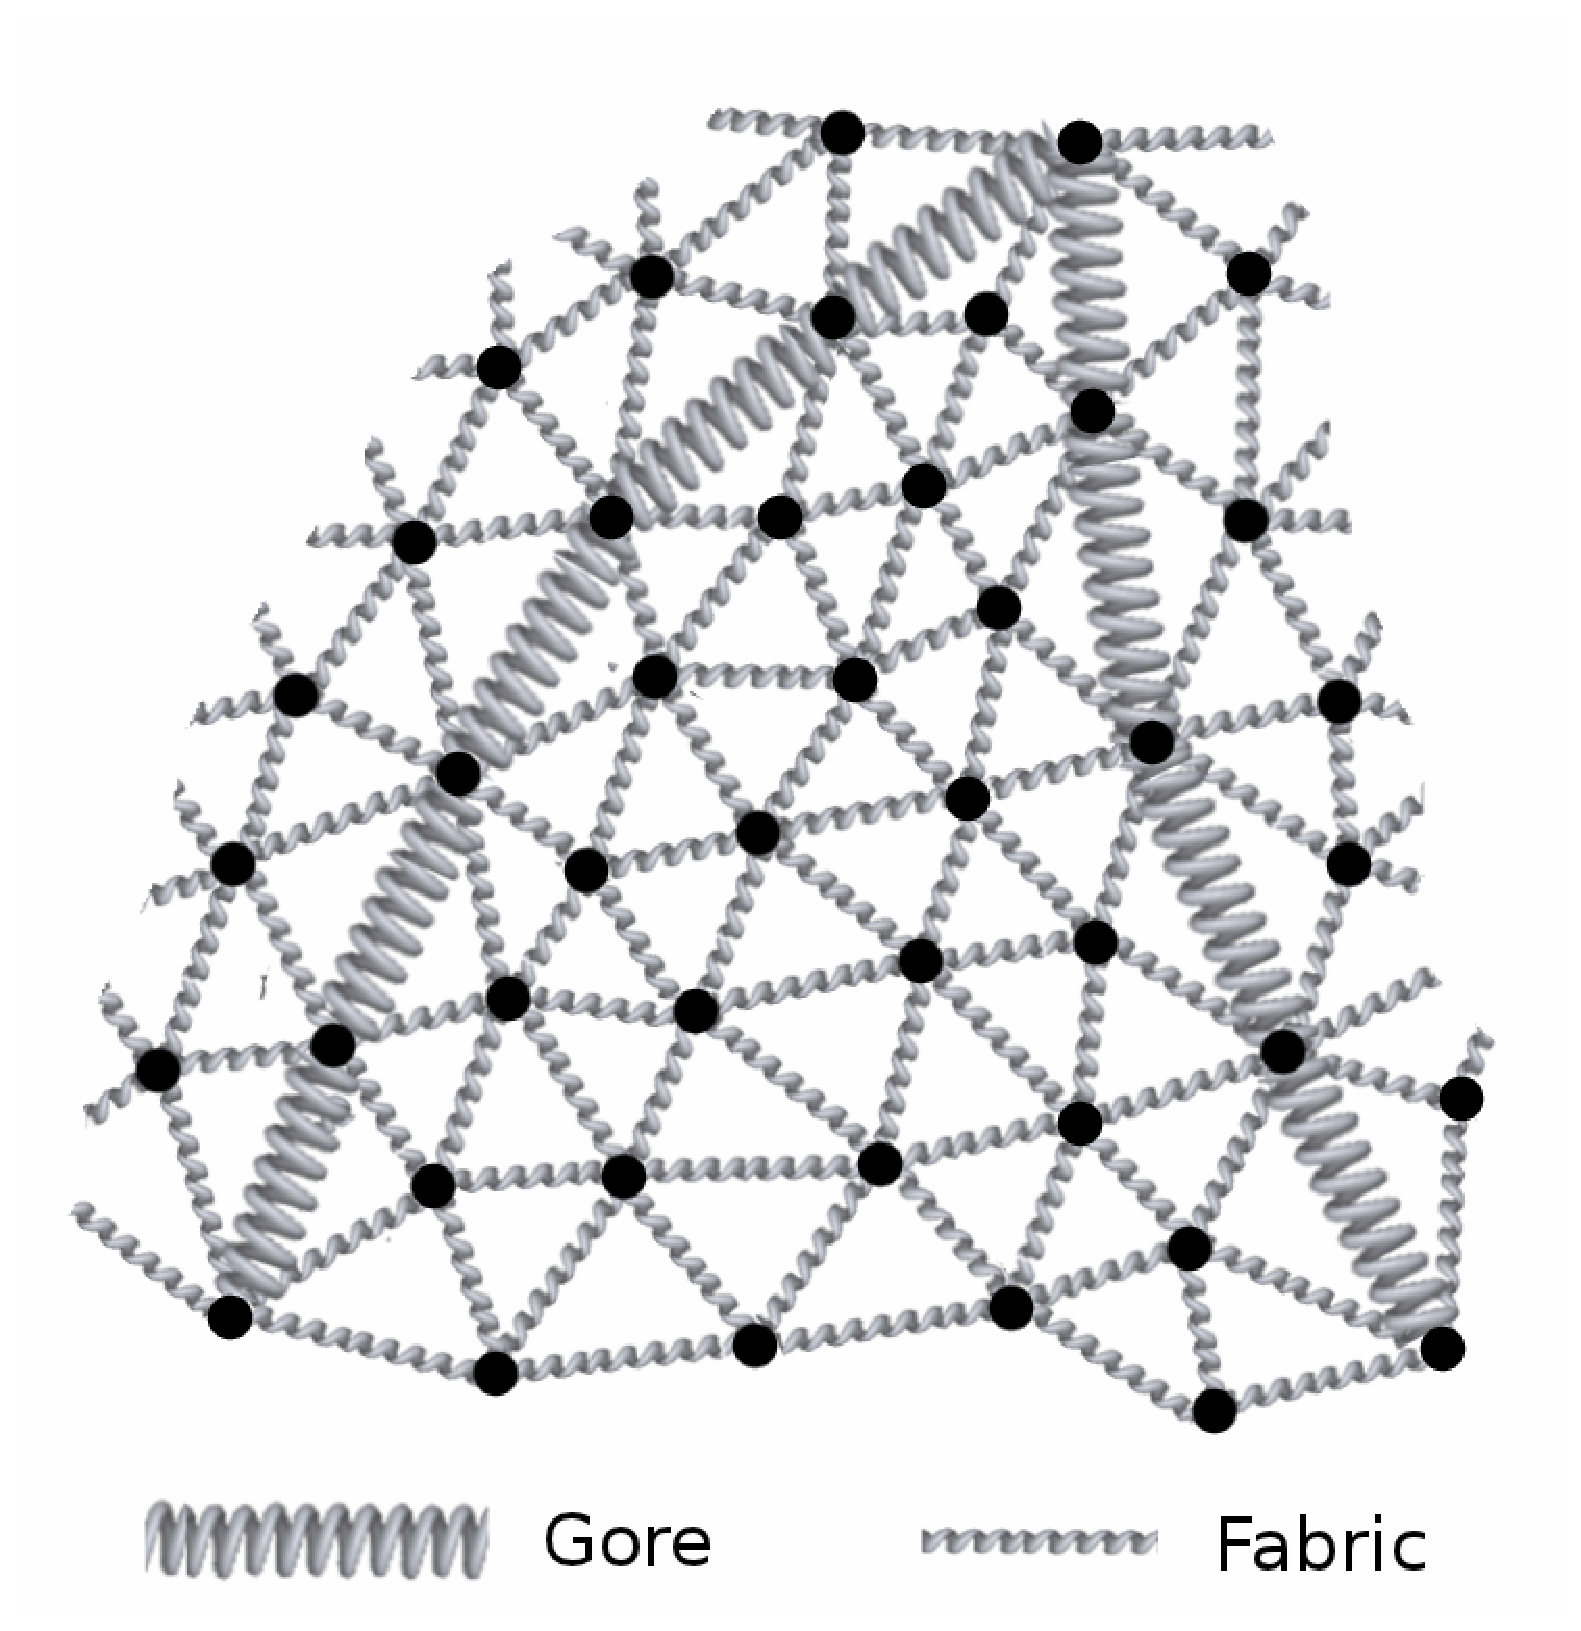
\epsfig{file=Figures/goremesh,width=0.55\hsize} \end{tabular} \caption{The
spring model on a triangulated mesh. Each vertex point in the mesh represents a
mass point with point mass $m$. Each edge of a triangle has a tensile stiffness.
With the equilibrium lengths set during the initialization, the changing length
of each side exerts a tensile spring force on the two neighboring vertices in
opposite directions.  Each angle of a triangle has an angular stiffness which is
set during the initialization. An additional tensile force is generated when the
the angle is changed. Gore boundaries are modeled by curves with higher tensile
stiffness.} \label{fig:goremesh} \end{figure}

Numerical implementation and testing have shown that such model is robust and
conforms with both the Young modulus and Poisson ratio of a given fabric
material. \Fig{fig:goremesh} demonstrates the mesh structure of such model.
In many literatures \cite{}, the internal force is decomposed to several parts,  
such as stretch forces, shear forces and bend forces. Our model is based on the 
formulation for elastic membrane, and thus only the in-plane forces are considered. 
The bend forces are relatively small comparing to the the other forces, so 
that is neglected in the current model.

\subsection{Additional Forces and Damping function}
In order to interact with the environment, we also added external forces, such as gravity 
and air-drag, to the internal forces. The gravity force is a constant force, and thus easy to implement:
\begin{equation}
\vect{f}_{g,i} = m_i \vect{g}
\end{equation}
An accurate calculation of air-drag should include both the velocity shear (friction drag) and the stress (pressure drag) to the surface. However, since calculating the friction drag requires substantially more computational resources to resolve the boundary layer and its contribution to the drag force is minor in comparison with the pressure drag for the bluff body \cite{}, we have followed \cite{KalroTezduyar2000} to neglect the friction forces in the  current model, then the air-drag is formulated on a per-point basis:
\begin{equation}
\vect{f}_{p,i} = \sigma(p_i^- - p_i^+)\vect{n} \label{eq:drag}
\end{equation}
where $p_i^-$ and $p_i^+$ are the pressure of point $i$ on lower and upper sides of the canopy, $\sigma$ is the mass density of canopy per unit area, and $\vect{n}$ is the unit normal vector pointing from lower to upper side of the canopy. The pressure $p^-$ and $p^+$ are calculated by making use of the left state and right state of the interface point in the front tracking method.

Robust dynamic cloth simulation is critically dependent on well-chosen damping forces \cite{}. A strong damping force must be applied to the spring system with strong stretch force to prevent anomalous in-plane oscillations. However, this strong damping force should confine itself solely to damping in-plane motions without affecting other forces. In previous literatures \cite{}, the in-plane damping force for point $i$ is chosen as:
\begin{equation}
\vect{f}_{d,i} = -k_d m_i\sum_{j \neq i}(\vect{v}_i - \vect{v}_j)^T\vect{e}_{ij}\vect{e}_{ij}
\label{eq:damping_1} 
\end{equation}
It is tempting to formulate a damping function as above. However, this damping function only works for the case with fabric surface solely and gives nonsensical results for the case involving fabric connecting with strings. An alternative method is \cite{Terzopoulos87, Terzopoulos88, Carignan1992, Platt1988}'s treatment of cloth that used a simple viscous damping function which dissipated kinetic energy. We improve this method by subtracting the damping function with the external impulses, so that its influence on the external forces can be excluded:
\begin{equation}
\vect{f}_{d,i} = -k_d m_i(\vect{v}_i-I_{ext,i})
\end{equation}
where $I_{ext,i}(t,\vect{x}_i) = \int_0^t (\vect{f}_{g,i} + \vect{f}_{p,i}) dt$.
This method works well for all our cases including the joint fabric and strings, and produces visually appealing results. One problem of this method is that a linear function of velocity does not match the quartic energy functions of the continuum formulation \cite{Baraff1998}, but will put this as future studies in the new paper.
 
\subsection{Fluid-fabric Coupling}
As discussed above, the fluid affects the motion of parachute canopy through the pressure drag and friction drag on the surface. In the opposite side, the parachute canopy is treated as an internal moving boundary for the fluid field. In this dissertation, the fluid field is modeled with incompressible Navier-Stokes equation, whose dynamics is controlled by the boundary conditions. The external boundary, such as inflow, outflow, periodic and wall boundaries can be handled trivially by defining an appropriate boundary condition following the underlying numerical scheme. As for the internal boundaries, the parachute canopy, we use the normal velocity computed from the ODEs of the spring system as the boundary value. Therefore, at each time step, we solve a Dirichlet boundary problem for the Naiver-Stokes equation.

\section{Turbulence modeling} \label{sec:turbulence}
Due to large Reynolds number (which is in the magnitude of several millions for a full-scale parachute canopy\cite{Johari2005}), turbulence model is required to accurately predict the the motion of the parachute system. A simple approach is to apply an appropriate eddy viscosity models based on the Reynolds Averaged Navier-Stokes (RANS) equation. The
hydrodynamic behavior of a turbulent incompressible fluid is governed by the
RANS equations for the mean velocity $\vect{u}$ and pressure $p$ 
\begin{equation}
\begin{aligned} 
\frac{\partial \vect{u}}{\partial t}+\vect{u}\cdot\nabla \vect{u} = -\nabla p +
\nabla\cdot((\nu+\nu_T)[\nabla \vect{u} + \nabla \vect{u}^T])\\ 
\nabla\cdot \vect{u} = 0
\end{aligned}\label{eq:NS} \end{equation} 
where $\nu$ is the kinematic viscosity and $\nu_T$ is the turbulent eddy viscosity which approximates the turbulent fluctuations.

We compared two eddy viscosity models, the Baldwin-Lomax model and the
$k-\varepsilon$ model.  In the Baldwin-Lomax \cite{Bldwin78} algebraic model,
$\nu_T = l_m^2\Omega$, where $l_m$ is the mixing length specified with a damping
function and $\Omega$ is the modulus of the mean rate of rotation tensor.  The
Baldwin-Lomax model is reliable since it seldom produces completely unphysical
results. Therefore, we adopt this model as the first step to test the effect of
turbulence on the fluid flow surrounding the parachute canopy. However, this
simple model tends to over-predict separation regions, thus not suitable for the
region around parachute canopies. A more realistic one is the RANS-based
turbulence model, or the $k-\varepsilon$ model family, which automatically
calculate the turbulence length scale \cite{wilcox1998turbulence}.  In standard
$k-\varepsilon$ model, the eddy viscosity is defined as \begin{equation} \nu_T =
C_{\mu}\frac{k^2}{\varepsilon}, \label{eq:nuT} \end{equation} where $k$ is the
turbulence kinetic energy and $\varepsilon$ is the dissipation rate. To compute
$k$ and $\varepsilon$, two additional convection-diffusion-reaction equations
are needed: \begin{equation} \frac{\partial k}{\partial
t}+\nabla\cdot(kU-(\nu+\frac{\nu_T}{\delta_k})\nabla k) =P_k - \varepsilon
\label{eq:k} \end{equation} \begin{equation} \frac{\partial
\varepsilon}{\partial t}+\nabla\cdot(\varepsilon U
-(\nu+\frac{\nu_T}{\delta_\varepsilon})\nabla \varepsilon)
=\frac{\varepsilon}{k}(C_1P_k-C_2\varepsilon) \label{eq:eps} \end{equation}
where $P_k = \frac{\nu_T}{2}|\nabla U + \nabla U^T|^2$ is the production of
turbulent kinetic energy. For the standard $k-\varepsilon$ model, the default
values of the involved empirical constants are: $C_\mu = 0.09$, $C_1 = 1.44$,
$C_2=1.92$, $\delta_k=1.0$, $\delta_{\varepsilon}=1.3$.  Although simple and
efficient, the standard model is unable to capture the effects of smaller scales
of motion due to its single turbulence length scale.  In order to account for
the different scales of motion, a mathematical technique called Re-Normalization
Group (RNG) method \cite{yakhot1992renormalization} is used to derive a
turbulence model similar to the standard one, resulting in a modified form of
the $\varepsilon$ equation: \begin{equation} \frac{\partial
\varepsilon}{\partial t}+\nabla\cdot(\varepsilon U
-(\nu+\frac{\nu_T}{\delta_\varepsilon})\nabla \varepsilon)
=\frac{\varepsilon}{k}(C_1P_k-C^*_2\varepsilon) \label{eq:RNG} \end{equation}
\begin{equation} C^*_2=C_2+\frac{C_{\mu}\eta^3(1-\eta/\eta_0)}{1+\beta\eta^3}
\end{equation} $\eta = kS/\varepsilon$, $S$ is the modulus of the mean rate of
strain tensor.  The coefficients are derived explicitly in the RNG procedure and
for completeness, we list here as: $C_\mu = 0.0845$, $C_1 = 1.42$, $C_2=1.68$,
$\delta_k=0.7194$, $\delta_{\varepsilon}=0.7194$.

The implementation of $k-\varepsilon$ model makes no difference in solving other
convection-diffusion-reaction equations, except two distinctions.  First, one
must specify an appropriate boundary condition at reflecting wall for the
velocity and two turbulence parameters. Due to extremely high Reynolds number in
parachute simulation, it is worthwhile using the wall functions to bridge the
viscosity-affected region and the fully-turbulent region in order to avoid the
need for high resolution of strong velocity gradients
\cite{kuzmin2007implementation}. Another task is to avoid loss of positivity of
$k$ and $\varepsilon$ due to computational errors.  This can be achieved by
keeping the coefficients positive for the linearized equations without changing
any primitive variables \cite{lew2001note}. Figure \ref{fig:keps} displays the
viscosity and velocity streamline computed with RNG $k-\varepsilon$ model.

\begin{figure}[!ht] \centering \begin{tabular}{cc}
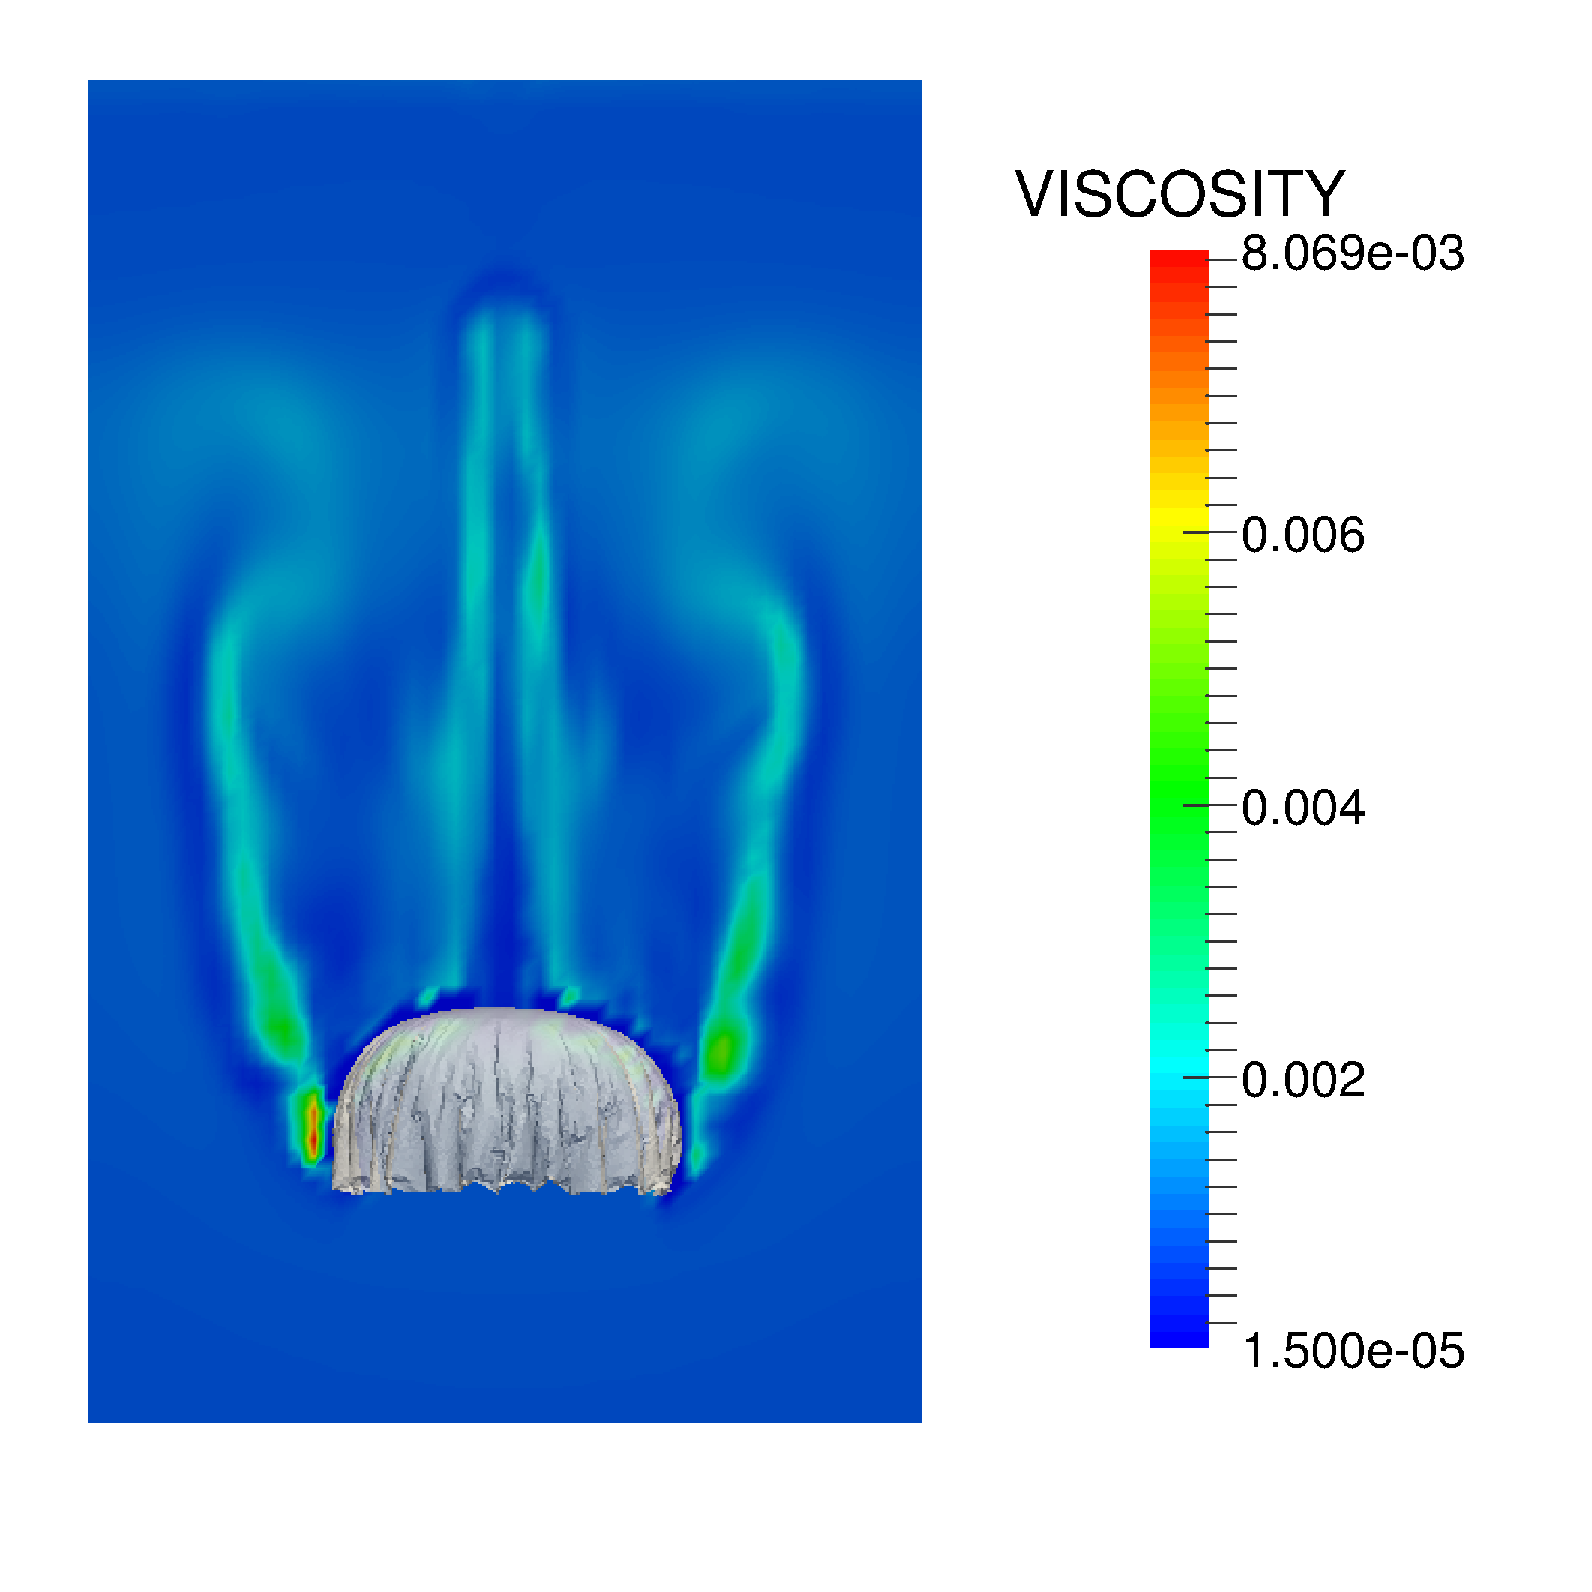
\epsfig{file=Figures/viscosity_rng,width=0.45\hsize} &
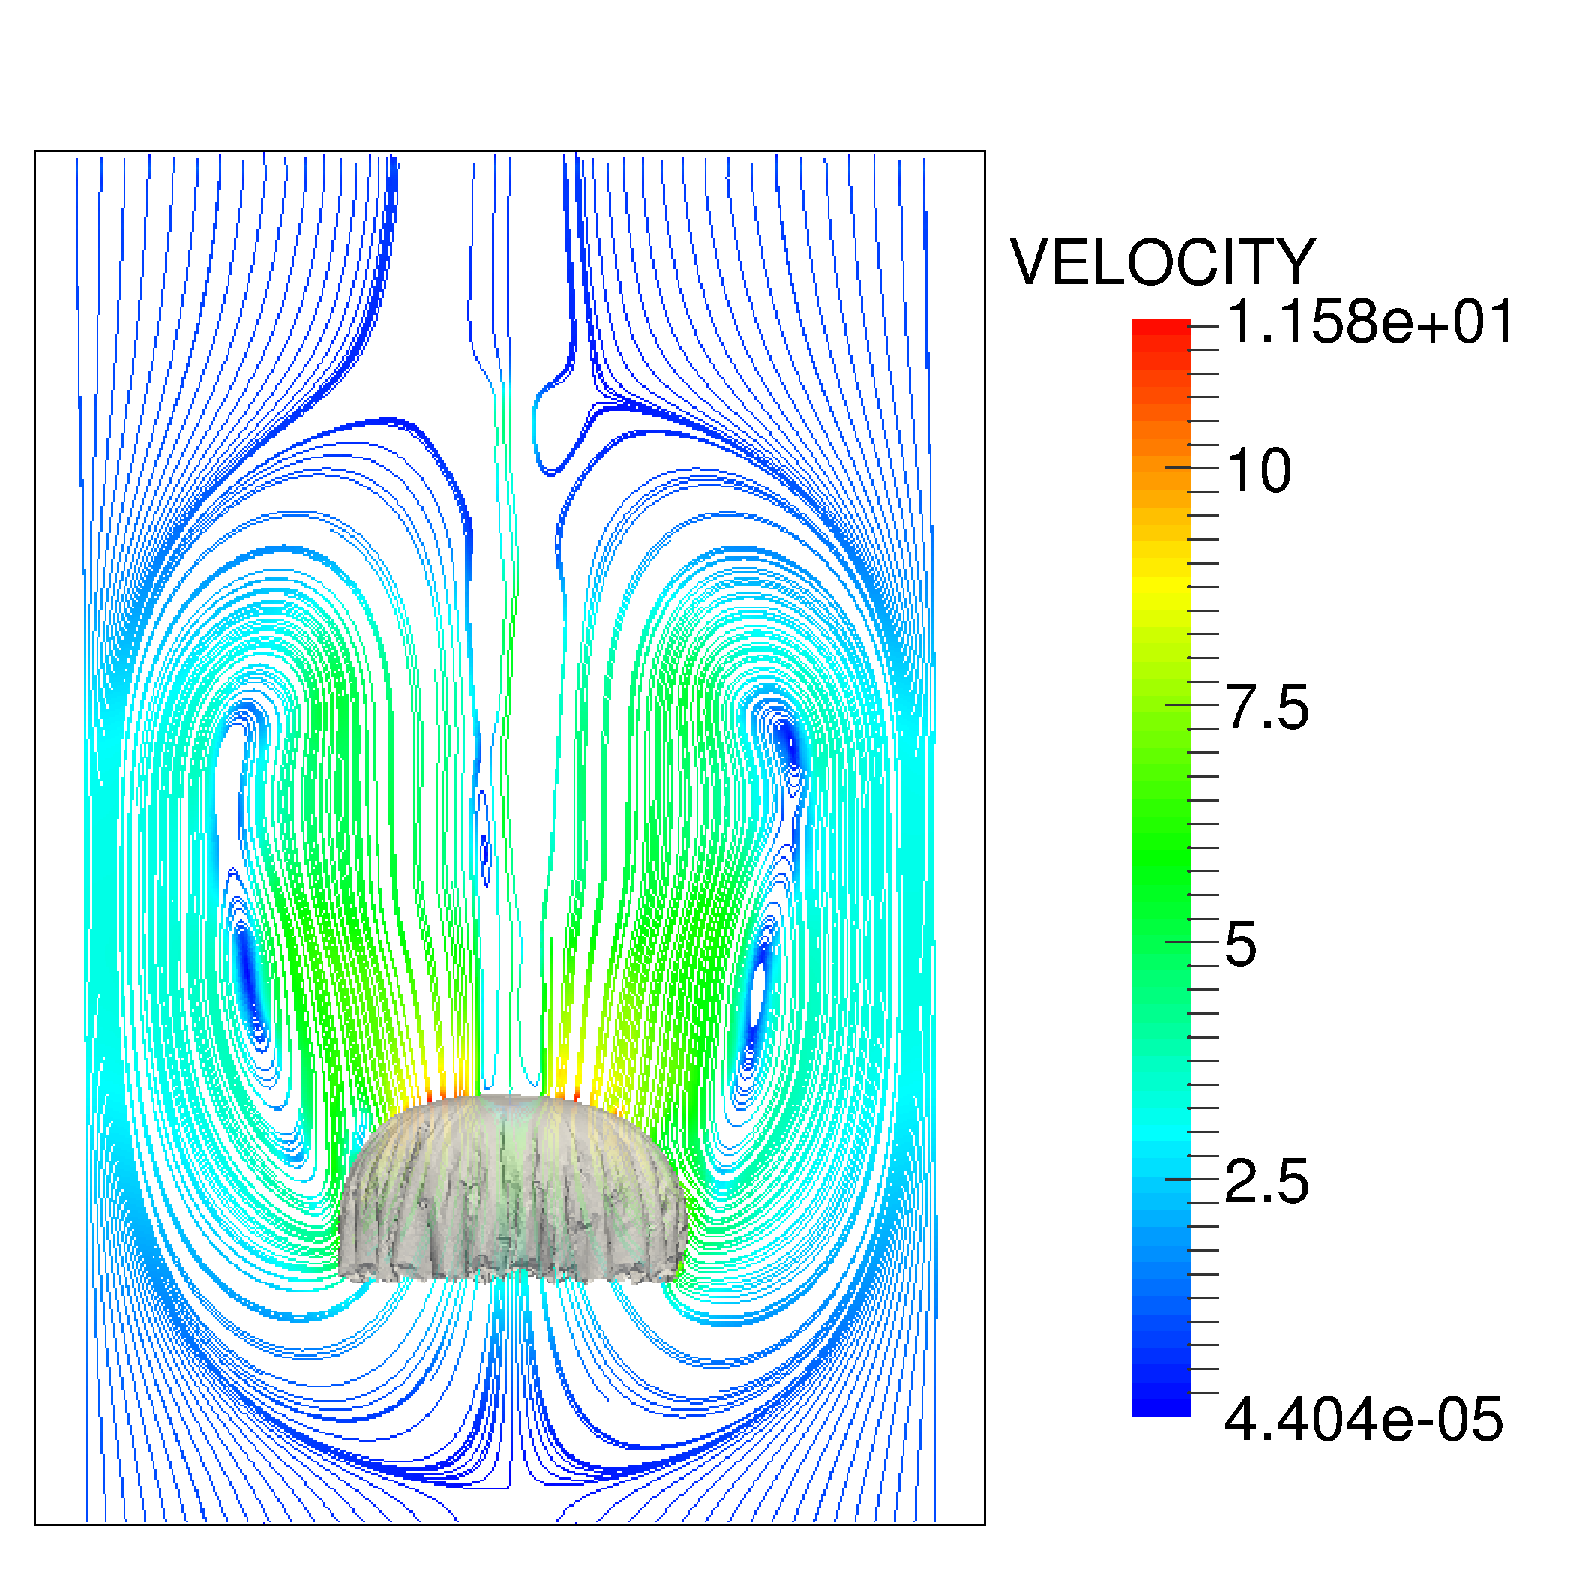
\epsfig{file=Figures/streamline_rng,width=0.45\hsize} \end{tabular}
\caption{Viscosity and streamline around parachute computed by RNG
$k-\varepsilon$ model \label{fig:keps}} \end{figure}

\subsection{Porosity modeling}
We consider an incompressible fluid in a $d = 2, 3$
dimensional bounded domain $\Omega$ during the time interval $(0,T)$. A porous
interface $\Gamma \subset R^{d-1}$ divides domain $\Omega$ into two subdomains
$\Omega^-$ and $\Omega^+$, that is
\begin{equation} \Omega = \Omega^+ \cup
\Gamma \cup \Omega^- \end{equation} The fluid velocity $\mathbf{u} = (u,v,w)$ and
pressure $p$ is determined by \Eq{eq:NS}.
The fabric porosity is simulated with the pressure jump condition at the interface:

\begin{eqnarray} \label{jumpcond} {[p]}_{\Gamma} &=& \alpha
\mathbf{u}_\Gamma\cdot \mathbf{n} + \beta |\mathbf{u}_\Gamma\cdot \mathbf{n}|
\mathbf{u}_\Gamma\cdot \mathbf{n} \\
{[u]}_{\Gamma} &=& 0 \end{eqnarray}
where $[p]_{\Gamma}=p^+ - p^-$ is the
pressure drop across the interface $\Gamma$; $p^+$ and $p^-$ are the pressure in
$\Omega^+$ and $\Omega^-$ respectively; $\mathbf{n}$ is the local unit normal
vector at the interface; $\mathbf{u}_\Gamma$ is the relative velocity between
interface and fluid field at the interface location. For the two parameters in
\Eq{jumpcond}, $\alpha$ is the viscous porosity coefficient and $\beta$ presents
the inertial porosity coefficient. $\beta \neq 0$ is used in the case of
turbulent flow with high Reynolds number.  Note that the sign of the subdomains
is decided by the normal vector of surface triangles which points from
$\Omega^+$ to $\Omega^-$.  In our application of parachute simulation, the
interface is an open surface, which means that $\Omega^+$ and $\Omega^-$ are
connected. Therefore $\Omega^+$ and $\Omega^-$ is only a valid concept locally
for the immediate vicinity of the fabric surface.

The interaction between fluid and fabric surface structure is handled by the
impulse method \cite{KimLiLi12} on the \FronTierp platform. The jump condition
\Eq{jumpcond} is considered by coupling the GFM with the finite difference
scheme at the projection step. We use the pressure-Poisson version of
projection method because the jump condition can be applied directly to the
Poisson equation.

Consider the computational domain $[L_x,U_x]\times[L_y,U_y]\times[L_z,U_z]$
which is discretized into $N_x\times N_y\times N_z$ cells of size $\Delta
x\times\Delta y\times\Delta z$. Let $\mathbf{u}^n_{ijk}$ represent the
numerical solution of velocity field at grid node  $\mathbf{x}_{i,j,k} =
[L_x+(i+0.5)\Delta x,L_y+(j+0.5)\Delta y, L_z+(k+0.5)\Delta z]$ at time $t^n =
n\Delta t$ and an analogous definition holds for the pressure $p^n_{ijk}$ ($i =
0,1,2,...,N_x-1$, $j = 0,1,2,...,N_y-1$, $k = 0,1,2,...,N_z-1$). The standard
pressure-Poisson version of projection method consists of the following steps:

Step 1: Compute the tentative velocity
\begin{eqnarray}
\frac{\mathbf{u}^*-\mathbf{u}^n}{\Delta t}+
[(\mathbf{u}\cdot\nabla_h)\mathbf{u}]^{n+1/2}
=\frac{\mu}{2\rho}\Delta_h(\mathbf{u}^*+\mathbf{u}^n)\\ B(\mathbf{u}^*) = 0,
\end{eqnarray} here $B(\cdot) = 0$ is the boundary condition for $\mathbf{u}$,
$[(\mathbf{u}\cdot\nabla_h)\mathbf{u}]^{n+1/2}$ is computed by the WENO scheme
\cite{WENO96} for the advection equation from $t_{n-1}$ to $t_{n}$ and then
extrapolated to $t_{n+1/2}$ \cite{KimMoin85}.

Step 2: Projection step
\begin{equation} \frac{1}{\rho}\Delta_h p^{n+1/2} =
\nabla_h\cdot \mathbf{u}^*/\Delta t \label{proj} \end{equation}

Step 3: Update new velocity
\begin{equation} \mathbf{u}^{n+1} = \mathbf{u}^* -
\frac{\Delta t}{\rho}\nabla_h p^{n+1/2} \label{newvel} \end{equation}
where
\begin{eqnarray} \label{divU} \nabla_h\cdot u =
\frac{u_{i+1,j,k}-u_{i-1,j,k}}{2\Delta x} +
\frac{v_{i,j+1,k}-v_{i,j-1,k}}{2\Delta y} +
\frac{w_{i,j,k+1}-w_{i,j,k-1}}{2\Delta z}\\ \label{gradP} \nabla_h p =
[\frac{p_{i+1,j,k}-p_{i-1,j,k}}{2\Delta x},
\frac{p_{i,j+1,k}-p_{i,j-1,k}}{2\Delta y},
\frac{p_{i,j,k+1}-p_{i,j,k-1}}{2\Delta z}]\\    \label{lapP} 
\begin{aligned}
\Delta_h p = \frac{p_{i+1,j,k}+p_{i-1,j,k}-2p_{i,j,k}}{\Delta x^2} +
\frac{p_{i,j+1,k}+p_{i,j-1,k}-2p_{i,j,k}}{\Delta y^2} \\ \quad
+\frac{p_{i,j,k+1}+p_{i,j,k-1}-2p_{i,j,k}}{\Delta z^2} \end{aligned}
\end{eqnarray}

The pressure jump condition is implemented while discretizing the pressure
function. Since the derivative is not defined through the interface, therefore,
the method by Liu in \cite{liu2000boundary} for the variable coefficient
Poisson equation is used to discretize the Laplacian operator in \Eq{proj} and
the gradient operator in \Eq{newvel}.  Liu used level set function
\cite{osher1988fronts} to determine the sign of the domain. In the front
tracking framework, one can use the local normal vector to decide the sign of a
grid point in the computational domain since the interface is explicitly
represented by topologically connected marker points \cite{GliGroLi98}.  For
example in \Fig{grid}, when discretizing at grid point $p_a$ along the $x$
direction, the sign of this point is defined by the sign of $\Phi_a =
\mathbf{v}_a\cdot \mathbf{n}_{\Gamma}$.  Therefore, the sign of a grid point is
allowed to vary when discretizing along different directions.

\begin{figure}[] \centering
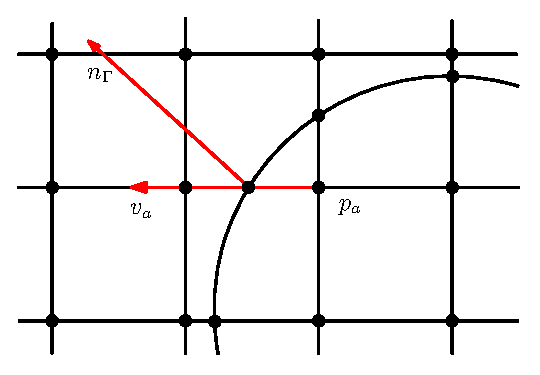
\includegraphics[width=0.6\textwidth]{Figures/grid.eps}
\caption{Numerical discretization near the interface. The plot
shows the algorithm for calculating
$\Phi_a = \mathbf{n}_\Gamma\cdot \mathbf{v}_a$, indicating the sign of the
domain at grid point $p_a$ when discretizing along $x$ direction. The normal
vector $\mathbf{n}_\Gamma$ at the interface-grid crossing is calculated by
\FronTierp with second order accuracy.}
\label{grid}
\end{figure}

Applying Liu's method to \Eq{proj} and \Eq{newvel}, we have
\begin{equation} \Delta_h p^{n+1/2}
= \nabla_h\cdot \mathbf{u}^*/\Delta t + F^x + F^y + F^z \label{newLap}
\end{equation} where $F^x = F^W + F^E$, $F^y = F^N + F^S$ and $F^z = F^T + F^B$.

\begin{equation} \label{newGrad} \mathbf{u}^{n+1} = \mathbf{u}^* - \Delta
t(\nabla_h p^{n+1/2} + G^x + G^y + G^z) \end{equation} where $G^x = G^W + G^E$,
$G^y = G^N + G^S$ and $G^z = G^T + G^B$.

The underlying idea to derive the additional terms in \Eq{newLap} and
\Eq{newGrad} is to define a ghost value for each grid node by imposing the jump
condition
\begin{equation} p_{i,j,k}^+ - p_{i,j,k}^- = a(\mathbf{x}_{\Gamma})
\label{disJump} \end{equation} where the indices "$\pm$" stand for the domain as
$\Omega^{\pm}$ and $a(\mathbf{x}_{\Gamma})$ is the pressure drop at the
interface location $\mathbf{x}_{\Gamma}$.  In consequence, every grid node has
two values for the solution, the real value and the ghost value.

According to the GFM, all the variables in the difference equation discretized
at point $\mathbf{x}_{i,j,k}$ should use the same domain indices as $\mathbf{x}_{i,j,k}$.
For example, if $\mathbf{x}_{i,j,k}$ is in domain of $\Omega^+$, then \Eq{gradP} becomes

\begin{equation} \label{ghostGradP} \nabla_h p =
[\frac{p^+_{i+1,j,k}-p^+_{i-1,j,k}}{2\Delta x},
\frac{p^+_{i,j+1,k}-p^+_{i,j-1,k}}{2\Delta y},
\frac{p^+_{i,j,k+1}-p^+_{i,j,k-1}}{2\Delta z}] \end{equation} and \Eq{lapP}
becomes
\begin{equation} \label{ghostLapP} 
\begin{aligned} \Delta_h p =
\frac{p^+_{i+1,j,k}+p^+_{i-1,j,k}-2p^+_{i,j,k}}{\Delta x^2} +
\frac{p^+_{i,j+1,k}+p^+_{i,j-1,k}-2p^+_{i,j,k}}{\Delta y^2} \\ \quad
+\frac{p^+_{i,j,k+1}+p^+_{i,j,k-1}-2p^+_{i,j,k}}{\Delta z^2} \end{aligned}
\end{equation}
In the case of $\Phi_{i,j,k} \cdot \Phi_{i+1,j,k} < 0$, that is
$\mathbf{x}_{i+1,j,k}$ is in the different domain from $\mathbf{x}_{i,j,k}$,
the ghost value $p^+_{i+1,j,k}$ should be replaced by its real value using the
jump condition \Eq{disJump}. It is easy to obtain
$F^E = -a(x_{\Gamma})/(\Delta x^2)$ and $G^E = -a(\mathbf{x}_{\Gamma})/(2\Delta x)$.

In the case of $\Phi_{i,j,k}\cdot\Phi_{i+1,j,k} > 0$, that is no interface exists between point $\mathbf{x}_{i,j,k}$ and $\mathbf{x}_{i+1,j,k}$, then $F^E = G^E = 0$.  The derivation of other terms is ignored here, since they are a straightforward extension of the above procedure.

n our situation, $a(\mathbf{x}_{\Gamma}) = [p]^n_{\Gamma} = \alpha
\mathbf{u}_{\Gamma}^n\cdot \mathbf{n} + \beta|\mathbf{u}_{\Gamma}^n\cdot
\mathbf{n}| \mathbf{u}_{\Gamma}^n\cdot \mathbf{n}$, where $\mathbf{u}_{\Gamma} =
\mathbf{u}_{interface} - \mathbf{u}_{fluid}$, $\mathbf{u}_{interface}$ is the
velocity of the interface point and $\mathbf{u}_{fluid}$ is obtained by using
the bilinear interpolation of the velocity field at the interface location.

Two sets of numerical tests are carried out to validate the numerical method.
The first set of tests is designed to study a steady incompressible flow
through a porous interface. The purpose of this numerical test is to verify the
implementation of our method. The pressure drop is expected to appear exactly
at the interface position as the model described in \Eq{jumpcond}.  The
computational domain is set to be $4m\times 0.4m\times 0.4m$ in the $x$, $y$,
$z$ directions respectively. The velocity is driven by an inflow with a
parabolic profile:
\begin{equation}
\mathbf{u}(x=0,y,z) = [16U_{max}yz(L_y - y)(L_z - z)/(L^2_yL^2_z),0,0]
\end{equation}
where $U_{max}$ is the maximum velocity at the center of the inlet, $L_y$ and
$L_z$ are the width of the channel in $y$ and $z$ directions.  An outflow
boundary condition together with the pressure $p = 0$ is applied to the outlet
at $x = 4m$ and a non-slip boundary condition of $\mathbf{u} = \mathbf{0}$ is
imposed for the remaining faces. The porous interface is orthogonal to the
streamline of flow and is placed at $x = 2m$. The coefficients in equation
\Eq{jumpcond} are set as $\alpha = 10 kgm^{-1}s^{-1}$ and $\beta = 0kgm^{-2}$.
The profiles of velocity and pressure at different positions are shown in
\Fig{fig:test1_profile}.

\begin{figure}[h] \centering
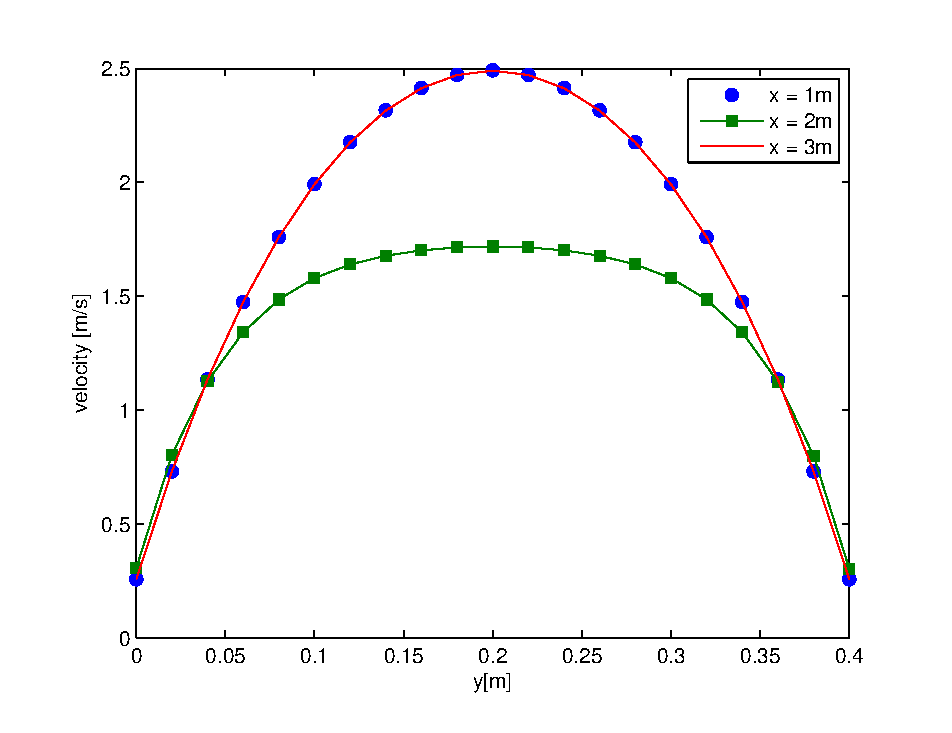
\includegraphics[width=0.49\columnwidth]{Figures/ucrs_profile}
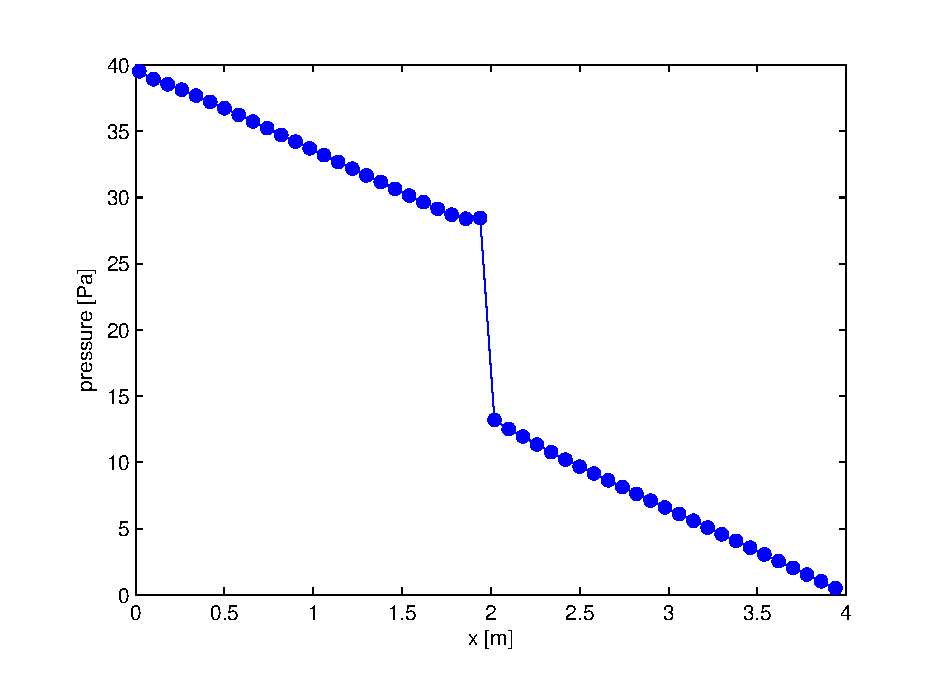
\includegraphics[width=0.49\columnwidth]{Figures/p_profile} \caption{(left)
Streamwise velocity profile at different sliced cross section and
(right) pressure along a axial direction with $y = 0.2m, z = 0.2m$. The plot
shows the velocity changes its profile as the fluid passes through the interface.
The pressure drop at the interface is well captured.}
\label{fig:test1_profile}
\end{figure}

In the second set of tests, a full scale model is used to simulate the response
of a realistic fabric surface in the channel flow.  The boundary conditions of
the computational domain are the same as the ones in the first test except that
the domain size is $30m\times 10m\times 10m$. The elastic fabric surface
located at $x = 5m$ is from the spring-mass model described in \cite{Shi2015}.
Thus the surface can be stretched or compressed due to the pressure drop at the
interface.  The fabric tested in the simulations resembles the properties of
MIL-C-7020 type III fabric \cite{ewing1978recovery} with density
$533.77kgm^{-3}$, Young's modulus $0.4309Gpa$. The values of viscous and
inertial parameters are $\alpha = 162kgm^{-1}s^{-1}$ and $\beta =
48.82kgm^{-2}$, which are calculated by fitting the experimental data using a
quadratic function.  The permeability velocity and the pressure drop are
measured by taking the average of the velocity and pressure drop over the
entire surface.  By imposing different values of inflow velocity, the
functional relationship between these two variables can be obtained. We
approximate the experimental data in \cite{ewing1978recovery} with formula
$[p]_{\Gamma} = \alpha U_n + \beta U_n^2$ and use it as the reference solution.
The results presented in \Fig{fig:curve} show that our model can successfully
reproduce the quadratic relationship observed in the experiments.

\begin{figure}[h] \centering
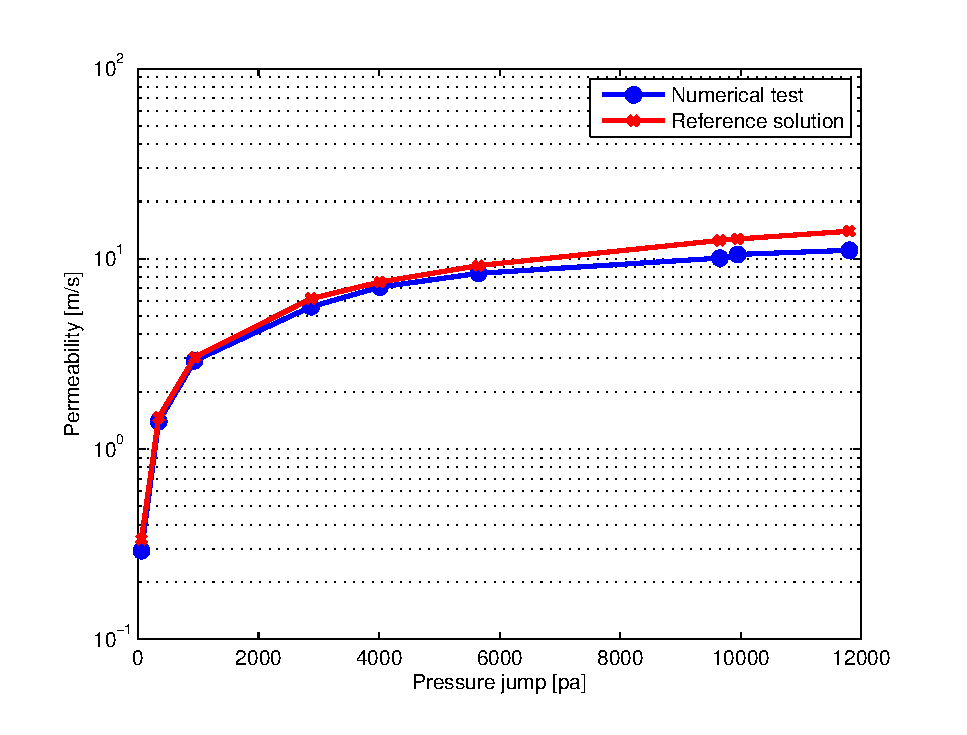
\includegraphics[width=1.0\columnwidth]{Figures/curve} \caption{Plot
of permeability velocity vs. pressure drop for the test case.
The numerical results show that there
is a quadratic relationship between the permeability velocity and
pressure drop. Such relationship is observed in the experiment (red line)}
\label{fig:curve} \end{figure}

\subsection{Collision treatment} 
Resolution of collision between different parts of
fabric surface or between fabric surface and rigid body is a very delicate
problem in mathematical algorithm and computational geometry.  In order to
resolve fabric collision during parachute inflation process, we have implemented
a collision handling function to detect and unwrap the surface in each time
step. The basic procedure of the algorithm is as follows:
\begin{itemize}
\item Select a collision time step size $\Delta t$ and set $t^{n+1}=t^{n}+\Delta t$
\item Record positions $\mathbf{x}^n$ of mass points at $t^n$
\item Compute spring mesh interior dynamics to get candidate positions
$\bar{\mathbf{x}}^{n+1}$
\item Calculate average velocity with
$\bar{\mathbf{v}}^{n+1/2} = (\bar{\mathbf{x}}^{n+1}-\mathbf{x}^n)/\Delta t$
\item Call collision solver to modify $\bar{\mathbf{v}}^{n+1/2}$ to obtain the
final mid-step velocity $\mathbf{v}^{n+1/2}$
\item Compute the final position
$\mathbf{x}^{n+1} = \mathbf{x}^n+\mathbf{v}^{n+1/2}\Delta t$
\item Advance the mid-step velocity $\mathbf{v}^{n+1/2}$ to $\mathbf{v}^{n+1}$ \end{itemize}
This method can guarantee no dynamic self-interference of cloth after a successful
call of the function. We coupled our collision handling function with the {\it
FronTier++} library. We also used algorithms and techniques such as the AABB
tree to accelerate the procedure, the impact zone method to reduce number of
iterations per step, and OpenMP to parallelize the traverse of the triangle
list.  Our algorithm can efficiently and robustly handle the fabric-fabric and
fabric-rigid body collision. We are still in the process of implementing and
testing the fabric-string and string-string collision.  \Fig{fig:collision}
shows the numerical results of fabric-rigid body collision.

\subsection{Inclusion of parachutists} 
The dimensions of parachutist or cargo are usually smaller than the parachute
canopy. However, when the fluid flows around the parachutist or cargo, it
generates vortex which will affect the stability of the inflating parachute
canopy.  Even in terminal descent regime, the turbulent flow passing through
the parachutist will reach the parachute and contribute to the instability of
the canopy motion.

Therefore the inclusion of parachutists will make numerical solution of
parachutes closer to reality and more convincing.  Figure \ref{fig:init_closer}
is amplification of the local mesh and connecting string chord to the cargo.

We added parachutist or cargo as a rigid body interacting with the surrounding
fluid flow, and the rigid body is connected to the parachute canopy through
string chords. In addition, we added the following components:

\begin{itemize}
\item Calculation of force and torque on the parachutist/cargo. This consists
of three parts: force of gravity, force exerted by the fluid flow and force
from each of the string chords. The force and torque will then be applied to
the center of mass of the parachutist for translational acceleration and
angular acceleration.

\item Propagation of the parachutist/cargo. The center
of mass motion and rotation about the center of mass are added to each marker
point representing the rigid body. The propagation must maintain the geometric
shape of the parachutist/cargo. This has perfect match with the Lagrangian
propagation of the front tracking method.
\end{itemize}

\begin{figure}[!ht] \centering
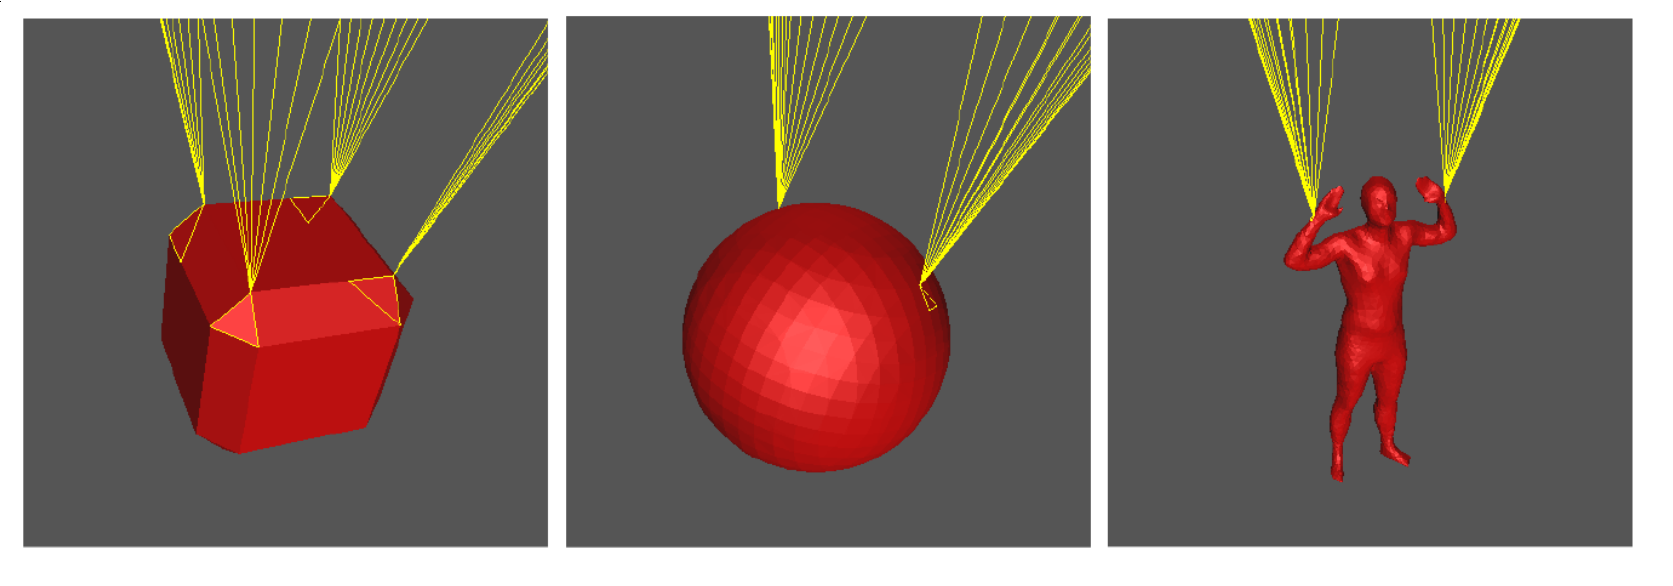
\includegraphics[width=6in]{Figures/parachutist-1.png} \caption{A closer look at
the parachutists.}\label{fig:init_closer} \end{figure}

Figure \ref{fig:G11-inflation} demonstrates the G11-parachute inflation at
different time. In this case, the parachutist is considered as a rigid body.

\begin{figure}[!ht] \centering \includegraphics[width=6in]{Figures/G11-box.eps}
\caption{The inflation process of G11-parachute with a cubic cargo.  The times
for each plot from the left to right are: t = 1.0 (left), t = 2.0 (middle), t =
3.0 (right), in second.} \label{fig:G11-inflation} \end{figure}

\subsection{Parallelism} 
The \FronTierp library offers functions for parallelized
operations of initialization and front propagation. On parallel platform, the
computational domain is divided into a partition of dimensions. A buffer
interface is attached at the boundary of each subdomain. After propagation of
the interface in each time step, the buffer surface is updated through exchange
of interface geometry and state data with the neighboring subdomains. For
parachute simulation, we use PETSc to solve for the Navier-Stokes equation in
both the advection and projection steps.  The parallelization of ODE solver for
the parachute canopy is more challenging.  It is parallelized through the OpenMP
or the GPU platform.

\begin{figure}[!ht] \centering \begin{tabular}{ccc}
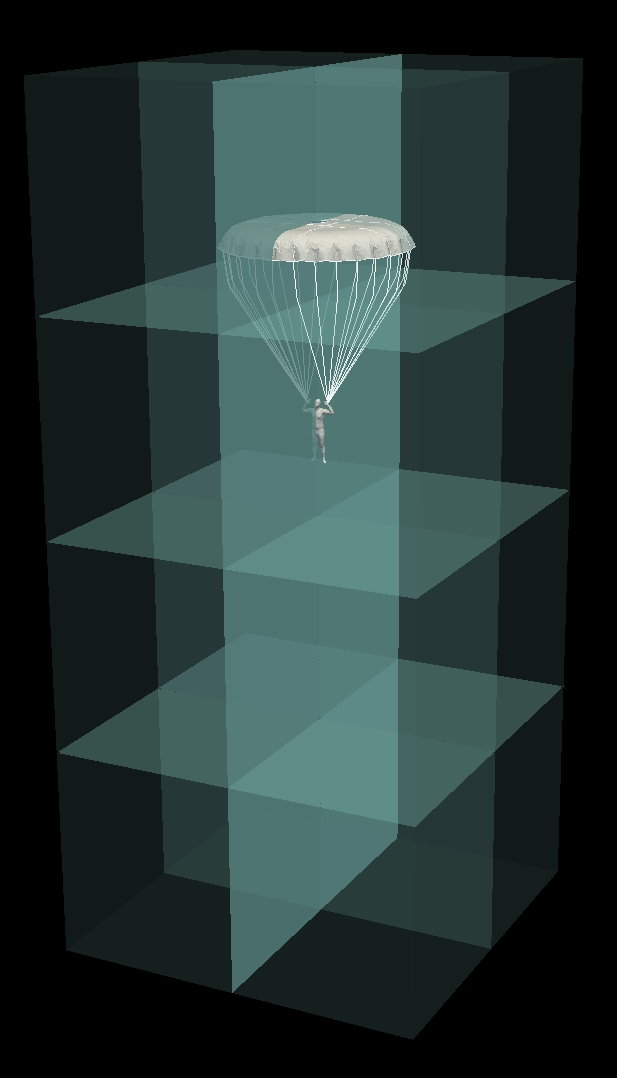
\epsfig{file=Figures/parallel-16-0,width=0.25\hsize}
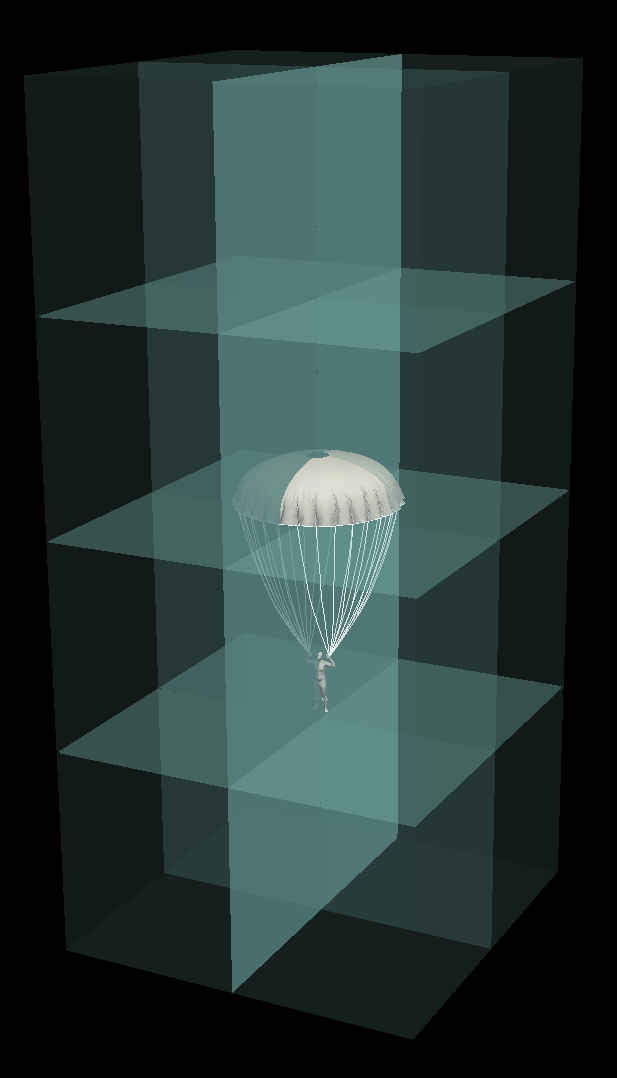
\epsfig{file=Figures/parallel-16-1,width=0.25\hsize}
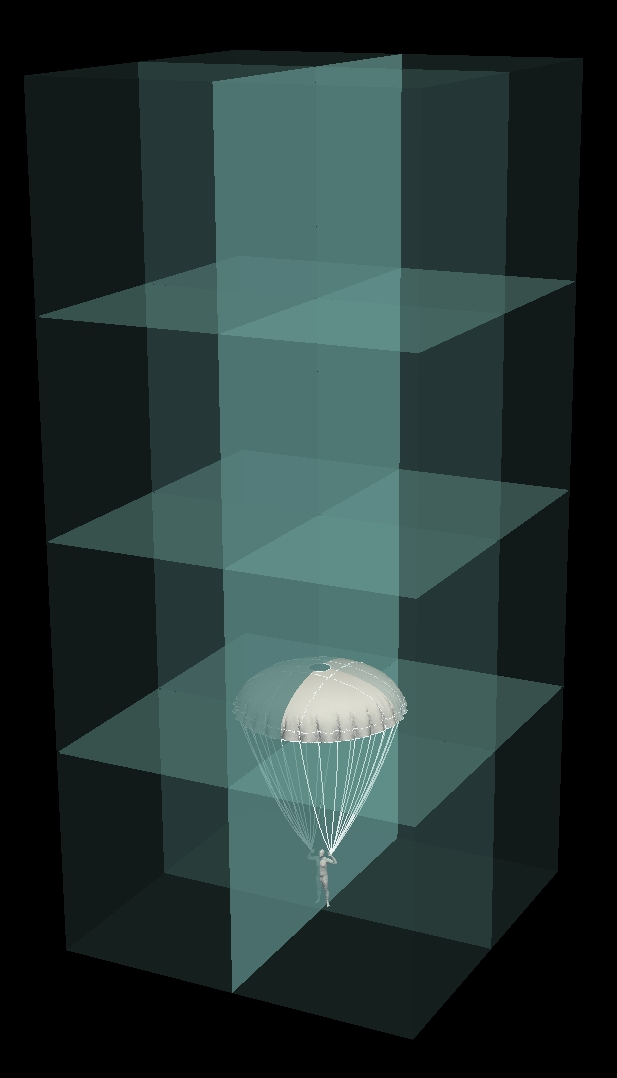
\epsfig{file=Figures/parallel-16-2,width=0.25\hsize} \end{tabular} \caption{
Parallel simulation of parachute descending on Dell Precision T7600 Workstation
with 16 subdomains. The neighboring subdomains are communicated via MPI while
the spring model is solved on OpenMP or GPU system.  The numerical algorithm is
capable of running on parallel computer with many processors but requires tuning
for efficiency and load balance.  \label{fig:parallel}} \end{figure}

Graphics Processing Unit (GPU) computing \cite{kirk2010programming} is to use
the GPUs together with CPUs to accelerate a general-purpose scientific and
engineering application.  GPU computing can offer dramatically enhanced
application performance by offloading computation-intensive portions of the
programming code to the GPU units, while the remainder of the code still runs on
the CPU.  Joint CPU/GPU applications constitute a powerful combination because
CPUs consist of a few cores optimized for serial processing, while GPUs consist
of thousands of smaller, more efficient cores designed for massive parallel
calculations.  Serial portions of the code with logical comparison run on the
CPU while floating point operation intensive parallel portions of the code run
on the GPU.

Our current strategy is to collect the point data to a sever processor and then
apply OpenMP or GPU solver in each of the sever nodes. This algorithm is not
efficient and does not scale linearly as the total number processors is
increased. We are testing several different alternatives and comparing pros and
cons of each method.

Global indexing is a new feature added to the \FronTierp computational library
for fluid structure interaction.  Since the original \FronTierp
\cite{DuFixGli05} deals with frequent surface mesh optimization and topological
reconstruction, its parallelization is based on the floating point matching.
The floating point matching is not completely reliable therefore more
complicated algorithms were implemented as the reinforcement.  For fabric-like
surface, especially when a spring-mass model is used, the inter-connectivity and
proximity of the interface marker points are static. Therefore, global indexing
is ideal for the parallel communication of the surface information and is now
employed in the work.  This new feature enables the parallel communication of
interface topology and geometry on a much more reliable and robust basis. It has
greatly reduced the run-time interruption due to bugs and efficiency in
geometrical and topological matching.

\section{Numerical Results}

\section{Summary and Conclusion}
